\subsection{System Overview}
Through the system overview diagram, in figure \ref{fig:system_overview}, it is possible to identify the main modules of the system to be developed, and how they interact. We can divide the system into two subsystems: the local system, which represents a lamp post, and the monitoring device, which can monitor a network of lamp posts.

\begin{figure}[ht]
	\centering
	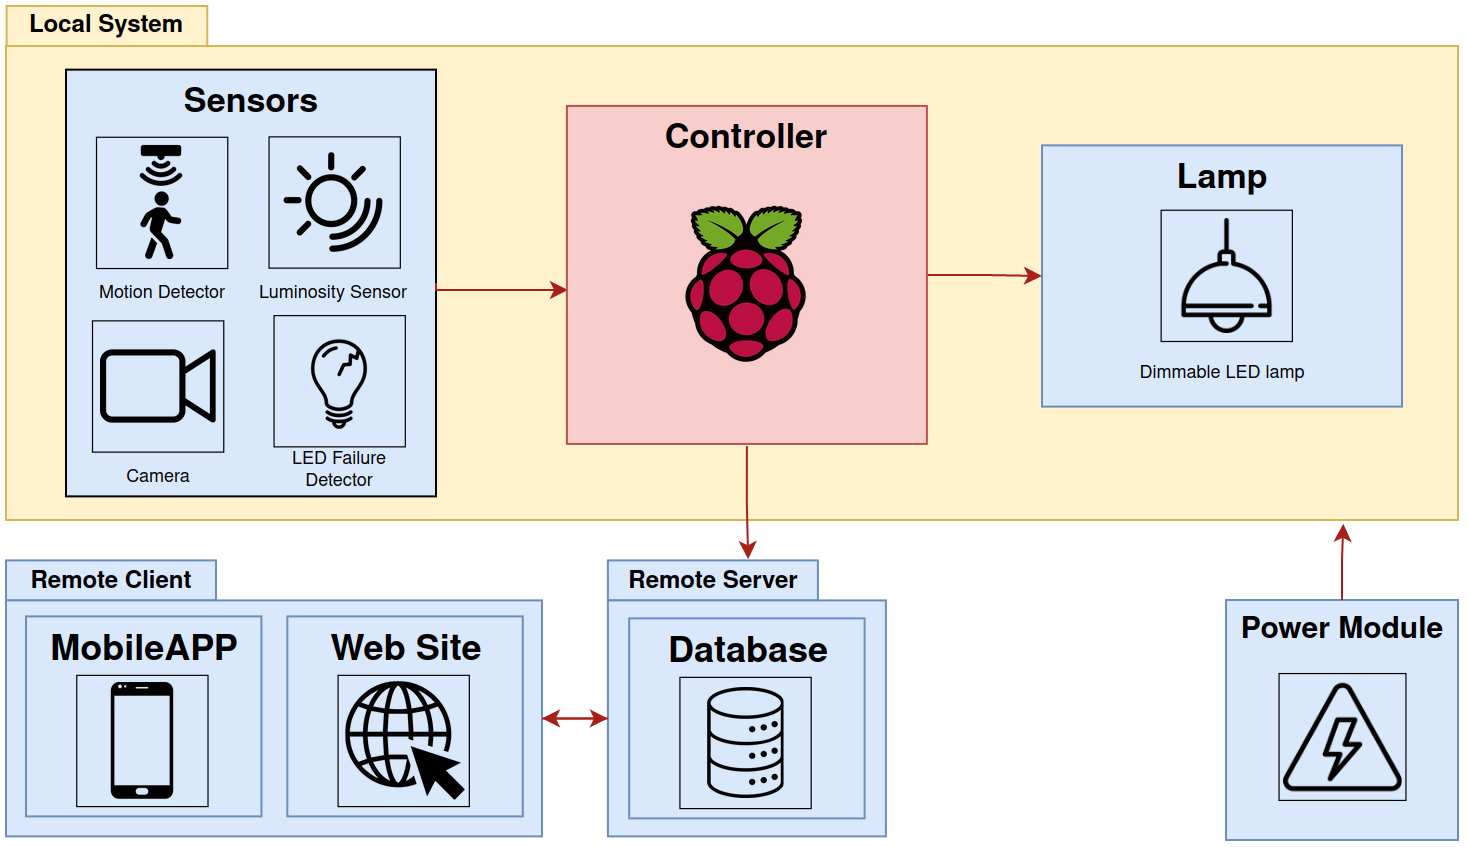
\includegraphics[width=1\textwidth]{system_overview}
	\caption{System Overview Diagram.}
	\label{fig:system_overview}
\end{figure}

The local system is composed of sensors, a controller and a lamp. Regarding the sensors, there will be a motion detector, to allow the detection of movement in the vicinity of the pole, and a light sensor, to detect the light conditions of the pole’s surroundings. The controller, through sensors information, controls the luminosity of the lamp and communicates via wireless with the monitoring device. The monitoring device exchanges data with a database, recording all information relating to each local system. This information can also be viewed and managed by a mobile application, which can be accessed by a person responsible for the street lamp network. Knowing that the public lighting network is directly related to the electrical network, this will be used to power local systems, such as the monitoring device.

\subsection{System Requirements and Constraints}

\subparagraph{Functional Requirements}
\begin{itemize}
	\item Sensors data acquisition				\item Motion detector
	\item Control of a street lamp
	\item Control a network of street poles		\item Wireless communication
	\item Access system information through a mobile application
\end{itemize}

\subparagraph{Non-Functional Requirements}
\begin{itemize}
	\item User friendly mobile application
	\item Ambient luminosity sensing
	\item Lower power consumption than actual street lights
	\item Soft Real-Time Embedded System
\end{itemize}

\subparagraph{Technical Constraints}
\begin{itemize}
	\item Buildroot
	\item C/C++ 
	\item Device Drivers
	\item Linux
	\item Raspberry Pi
	\item \ac{cps}
	\item Makefiles
	\item Pthreads
\end{itemize}

\subparagraph{Non-Technical Constraints}
\begin{itemize}
	\item Two members team
	\item Project deadline at the end of the semester
	\item Low budget
	
\end{itemize}

\section{Software Architecture}

\section{Hardware Architecture}
